\documentclass[11pt]{article}

\newcommand{\HWnum}{5} 
\newcommand{\StudName}{Timothy Holmes} % author
\newcommand{\CourseNum}{411}           % course number
\newcommand{\Subject}{PHY}

\usepackage{graphicx, amsmath, amssymb,fancyhdr}
\addtolength{\textwidth}{1.5in}
\addtolength{\oddsidemargin}{-2cm}
\addtolength{\evensidemargin}{-2cm}
\addtolength{\textheight}{1.6in}
\addtolength{\topmargin}{-0.7in}
\addtolength{\headsep}{-0.1in}
%\addtolength{\footskip}{-0.2in}
\pagestyle{fancy}
\cfoot{}
\lhead{\textbf{\Subject~\CourseNum~--- Homework~\HWnum}}
\rhead{\textbf{\StudName:~Page~\thepage}}

\addtolength{\parskip}{\baselineskip} % skips a line between paragraphs
\parindent 0in                        % no indent at start of paragraph

\newcommand{\dd}{\textrm{d}}
\usepackage{braket}
\usepackage{lipsum, babel}
\usepackage{blindtext}
\usepackage{graphicx}% Include figure files
\usepackage{dcolumn}% Align table columns on decimal point
\usepackage{bm}% bold math
\usepackage{listings}
\usepackage{listing}
\usepackage{supertabular}



\usepackage{color} %red, green, blue, yellow, cyan, magenta, black, white
\definecolor{mygreen}{RGB}{28,172,0} % color values Red, Green, Blue
\definecolor{mylilas}{RGB}{170,55,241}



\lstset{language=Python,%
    %basicstyle=\color{red},
    breaklines=true,%
    morekeywords={matlab2tikz},
    keywordstyle=\color{blue},%
    morekeywords=[2]{1}, keywordstyle=[2]{\color{black}},
    identifierstyle=\color{black},%
    stringstyle=\color{mylilas},
    commentstyle=\color{mygreen},%
    showstringspaces=false,%without this there will be a symbol in the places where there is a space
    numbers=left,%
    numberstyle={\tiny \color{black}},% size of the numbers
    numbersep=9pt, % this defines how far the numbers are from the text
    emph=[1]{for,end,break},emphstyle=[1]\color{red}, %some words to emphasise
    %emph=[2]{word1,word2}, emphstyle=[2]{style},    
}



\begin{document}
% -------------------------- BOD -------------------------- 

\title{Homework {\HWnum}}
\author{Timothy Holmes \\ \Subject~411 Electrodynamics I}

\maketitle

\section*{Problem 1}

Preferences in order:

\subsection*{(d) Waveguides}

I find this to be the most interesting topic because I enjoy to see when the fundamental side of physics meets the applied side. Seeing how the physics works into our everyday lives gives me a better grasp on the topic of study. I also enjoy topics that I am also able to write programs for and simulate, which implements the ability to change parameters on the fly to quickly understand the results. 

\subsection*{(b) Problem 7.2}

\subsection*{(e) Toy MHD}

\subsection*{(a) Model of the ionosphere}

\subsection*{(c) Problem 7.15}

\clearpage

\section*{Problem 2}

\begin{align*}
    \Phi &= 0 & \Vec{A} &= \hat{y}A_{0}sin(kx - \omega t)
\end{align*}

\subsection*{(a)}

$\Vec{E}$ is gave as 

$$
\Vec{E} = -\Vec{\nabla} \Phi - \frac{\partial \vec{A}}{\partial t}.
$$

Next, substitute the vector and scalar potential above. When $\Phi = 0$, the vector potential, is entered into the $\Vec{E}$ this part of the equation becomes $-\Vec{\nabla} 0 = 0$. The other portion of the equation, when entering the scalar potential, becomes $\partial/\partial t = \Vec{A} = \hat{y}A_{0}sin(k x - \omega t)$. Therefore the $\Vec{E}$ field becomes 

$$
\Vec{E} = -\frac{\partial }{\partial t} (\hat{y}A_{0}sin(k x - \omega t)).
$$

The partial derivative with respect to time is 

$$
-\frac{\partial }{\partial t} (\hat{y}A_{0}sin(k x - \omega t)) = \hat{y}A_{0}cos(t\omega - k x).
$$

Thus,

$$
\Vec{E} = \hat{y}A_{0}\omega cos(\omega t - k x).
$$

$\Vec{B}$ is gave as 

$$
\Vec{B} = \Vec{\nabla} \times \vec{A}.
$$

Substituting the scalar potential into the $\Vec{B}$ field gives

$$
\Vec{B} = \Big( \hat{x}\Big(\frac{\partial}{\partial x} \Big) + \hat{y}\Big(\frac{\partial}{\partial y} \Big) + \hat{z}\Big(\frac{\partial}{\partial z} \Big)\Big) \times (\hat{y}A_{0}sin(kx - \omega t)).
$$

The cross product is

$$
\Vec{B} = \frac{\partial}{\partial x} (\hat{z}A_{0}sin(kx - \omega t) + 0 - \frac{\partial}{\partial z}  (\hat{x}A_{0}sin(kx - \omega t).
$$

Taking the derivatives gives

\begin{align*}
    \frac{\partial}{\partial x} (\hat{z}A_{0}sin(kx - \omega t) &= (\hat{z}A_{0}k cos(\omega t - kx) & \frac{\partial}{\partial z}  (\hat{x}A_{0}sin(kx - \omega t) &= 0
\end{align*}

Thus,

$$
\Vec{B} = (\hat{z}A_{0}k cos(\omega t - kx))
$$

\subsection*{(b)}

Both waves are traveling in the $-x$ direction. The $\vec{E}$ field is polarized in the $\hat{y}$ direction and the $\vec{B}$ field is polarized in the $\hat{z}$ direction. Both the electric field and the magnetic field are propagating in the same direction and they are perpendicular to one another. 

\clearpage

\section*{Problem 3}

Consider the gauge transformation

\begin{align*}
    \vec{A'} &= \vec{A} + \vec{\nabla}\Lambda & \Phi' = \Phi - \frac{\partial \Lambda}{\partial t}
\end{align*}

Suppose you are given the potentials:

\begin{align*}
    \Phi(\vec{r}, t) &= 0 & \vec{A}(\vec{r}, t) &= -\frac{qt}{4\pi\epsilon_{0}r^{2}}\hat{r}
\end{align*}

and suppose the gauge function $\Lambda$ is given by

$$
\Lambda = -\frac{qt}{4\pi\epsilon_{0}r}
$$

\subsection*{(a)}

$\Vec{E}$ is gave as 

$$
\Vec{E} = -\Vec{\nabla} \Phi - \frac{\partial \vec{A}}{\partial t}.
$$

Substituting the scalar potential into the $\Vec{E}$ field gives

$$
\Vec{E} = 0 - \frac{\partial}{\partial t} \Bigg(-\frac{qt}{4\pi\epsilon_{0}r^{2}}\hat{r}\Bigg).
$$

The derivative with respect to time is 

$$
- \frac{\partial}{\partial t} \Bigg(-\frac{qt}{4\pi\epsilon_{0}r^{2}}\hat{r}\Bigg) = \frac{q}{4\pi\epsilon_{0}r^{2}}\hat{r} 
$$

Thus,

$$
\Vec{E} = \frac{q}{4\pi\epsilon_{0}r^{2}}\hat{r}
$$

$\Vec{B}$ is gave as 

$$
\Vec{B} = \Vec{\nabla} \times \vec{A}.
$$

Substituting the scalar potential into the $\Vec{B}$ field gives

$$
\vec{B} = \Bigg(\frac{\partial}{\partial r} \hat{r} + \frac{1}{r} \frac{\partial}{\partial \theta} \hat{\theta} + \frac{1}{rsin(\theta)}\frac{\partial}{\partial \phi} \hat{\phi}\Bigg) 
\times 
\Bigg(-\frac{qt}{4\pi\epsilon_{0}r^{2}}\hat{r}\Bigg)
$$

Since the scalar potential $\vec{A}$ does not have components $\theta$ or $\phi$, the partial derivatives with the respect to these components are just 0. Therefore, $r$ will be the only component that will survive. However, since this is a cross product and both terms have $\hat{r}$ and $\hat{r} \times \hat{r} = 0$, then

$$
\vec{B} = 0.
$$

\subsection*{(b)}

The gauge transformation for $\vec{A'}$ is gave above along with gauge function $\Lambda$. Substituting the gauge function $\Lambda$ into the gauge transformation $\vec{A'}$ along with the potential $\vec{A}$ gives

$$
\vec{A'} = -\frac{qt}{4\pi\epsilon_{0}r^{2}}\hat{r} - 
\Bigg(\frac{\partial}{\partial r} \hat{r} + \frac{1}{r} \frac{\partial}{\partial \theta} \hat{\theta} + \frac{1}{rsin(\theta)}\frac{\partial}{\partial \phi} \hat{\phi}\Bigg)
\frac{qt}{4\pi\epsilon_{0}r}.
$$

Since the gauge function $\Lambda$ does not have components $\theta$ or $\phi$, the partial derivatives with the respect to these components are just 0. Therefore, $r$ will be the only component that will survive. Taking the derivative of this is

$$
-\frac{\partial}{\partial r} \hat{r} \frac{qt}{4\pi\epsilon_{0}r} = \frac{qt}{4\pi\epsilon_{0}r^{2}}\hat{r}
$$

Therefore, the gauge transformation

$$
\vec{A'} = -\frac{qt}{4\pi\epsilon_{0}r^{2}}\hat{r} + \frac{qt}{4\pi\epsilon_{0}r^{2}}\hat{r}
$$

Thus, 

$$
\vec{A'} = 0 
$$

The gauge transformation for $\Phi'$ is gave above along with gauge function $\Lambda$. Substituting the gauge function $\Lambda$ into the gauge transformation $\vec{\Phi'}$ along with the potential $\Phi$ gives

$$
\Phi' = \frac{\partial}{\partial t} \Bigg(-\frac{qt}{4\pi\epsilon_{0}r}\Bigg).
$$

Taking the derivative with respect to time gives

$$
 \frac{\partial}{\partial t} \Bigg(-\frac{qt}{4\pi\epsilon_{0}r}\Bigg) = -\frac{q}{4\pi\epsilon_{0}r}
$$

Thus,

$$
\Phi' = -\frac{q}{4\pi\epsilon_{0}r}
$$

\subsection*{(c)}

Substituting the answers found in section (b) into the fields $\vec{B}$ and $\vec{E}$ will create the fields $\vec{E'}$ and $\vec{B'}$. Starting with $\vec{E'}$, this will become

$$
\Vec{E'} = -\Vec{\nabla} \Phi' - \frac{\partial \vec{A'}}{\partial t}
$$

where

\begin{align*}
    \vec{A'} &= 0 &
    \Phi' &= -\frac{q}{4\pi\epsilon_{0}r}.
\end{align*}

The field then becomes

$$
\Vec{E'} = -\Bigg(\frac{\partial}{\partial r} \hat{r} + \frac{1}{r} \frac{\partial}{\partial \theta} \hat{\theta} + \frac{1}{rsin(\theta)}\frac{\partial}{\partial \phi} \hat{\phi}\Bigg)  \Bigg(\frac{q}{4\pi\epsilon_{0}r}\Bigg).
$$

There are no $\theta$ or $\phi$ components in the $\Phi'$ expression. Therefore, the derivatives of these components with respect to $\Phi'$ will be zero. The only remaining term will be the $\hat{r}$ term where the derivative is 

$$
-\frac{\partial}{\partial r} \hat{r} \Bigg(\frac{q}{4\pi\epsilon_{0}r}\Bigg) = \frac{q}{4\pi\epsilon_{0}r^{2}} \hat{r}
$$

Thus,

$$
\Vec{E'} = \frac{q}{4\pi\epsilon_{0}r^{2}} \hat{r}
$$

$\Vec{B'}$ is gave as 

$$
\Vec{B'} = \Vec{\nabla} \times \vec{A'}.
$$

Since $\vec{A'} = 0$ and the cross product with with zero is zero, then

$$
\vec{B'} = 0.
$$

\subsection*{(d)}

$\vec{E}$ and $\vec{E'}$ are gave as

\begin{align*}
    \Vec{E} &= \frac{q}{4\pi\epsilon_{0}r^{2}}\hat{r} & \Vec{E'} &= \frac{q}{4\pi\epsilon_{0}r^{2}} \hat{r}
\end{align*}

while $\vec{B}$ and $\vec{B'}$ are gave as

\begin{align*}
    \Vec{B} &= 0 & \Vec{B'} &= 0.
\end{align*}

Therefore, the $\vec{B}$ values are the same and the $\vec{E}$ have the same values. This can automatically be figured out since the fields should not change with the gauge transformation. Physically, this looks like an Coulomb's law where $q$ is the source charge and $r$ is the distance of separation. 

\clearpage

\section*{Problem 4}

\subsection*{(a)}

The amplitude that describes the properties of linear superposition of different waves is calculated by

$$
A(k) = \frac{1}{\sqrt{2\pi}} \int_{-\infty}^{\infty} u(x,0)e^{-ikx}dx,
$$

where


\[ u(x,0) = \begin{cases} 
       Ne^{ik_{0}x} & for \; |x| < a \\
      0 & for \; |x| > a. \\
   \end{cases}
\]

Given the boundaries above in the piece-wise function and entering in the equation above, the integral becomes

\begin{align*}
A(k) &= \frac{1}{\sqrt{2\pi}} N \int_{-a}^{a} e^{-ix(k - k_{0})}dx \\\\
&= \frac{2Nsin(a(k - k_{0}))}{\sqrt{2\pi}(k - k_{0})}.
\end{align*}

Now, if $|A(k)|$ is squared the equation becomes

$$
|A(k)|^{2} = \frac{2N^{2}}{\pi}\frac{sin^{2}(a(k - k_{0}))}{(k - k_{0}^{2})}
$$

\clearpage

\subsection*{(b)}

\begin{figure}[h!]%
    \centering
    \subfloat{{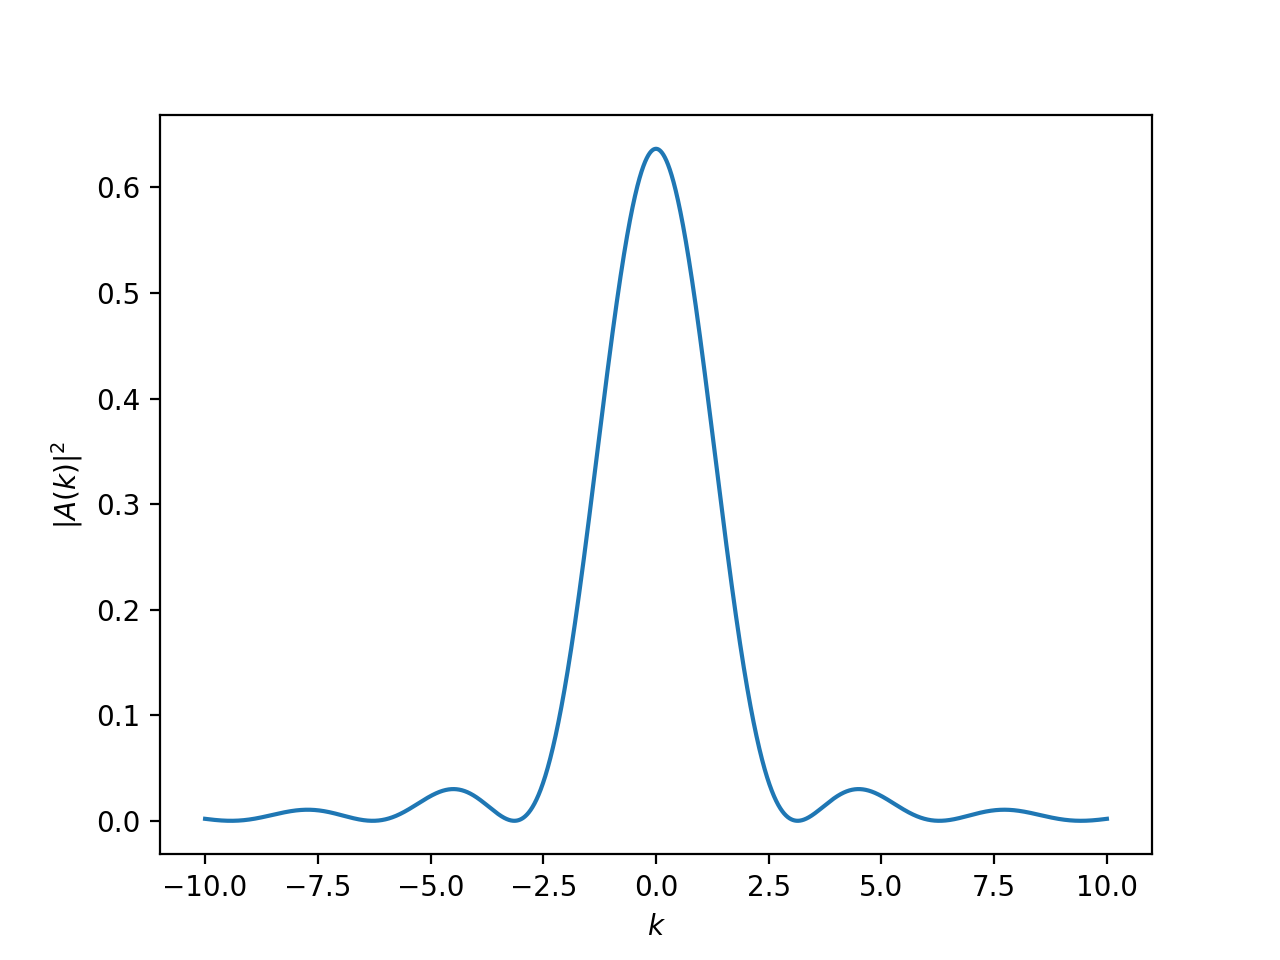
\includegraphics[width=13cm]{Figure_1.png} }}%
    \qquad
    \subfloat{{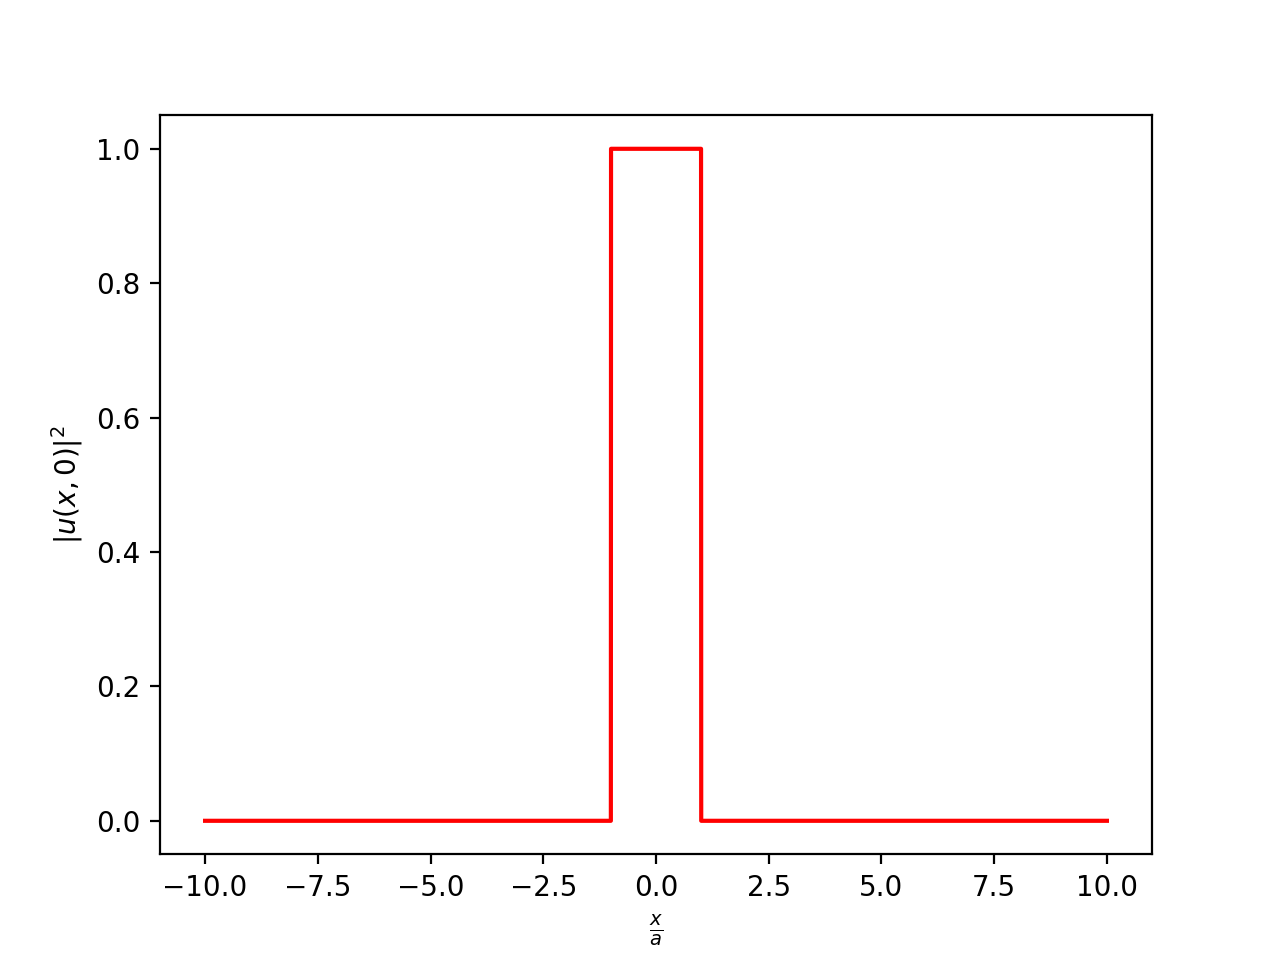
\includegraphics[width=13cm]{Figure_2.png} }}%
    \caption{Plot of  $|A(k)|^{2}$ vs $k$ in the top image (blue plot) and $|u(x, 0)|^{2}$ vs $x/a$ in the bottom image (red plot).}
    \label{fig:example}%
\end{figure}

\clearpage

\section*{Appendix}

\subsection*{$|A(k)|^{2}$ and $|u(x, 0)|^{2}$ Plot}
\lstinputlisting{homework5.py}

\clearpage

% -------------------------- EOD -------------------------- 
\end{document}